\documentclass[letterpaper,10pt]{article}
\usepackage[top=2cm, bottom=1.5cm, left=1cm, right=1cm]{geometry}
\usepackage{amsmath, amssymb, amsthm,graphicx}
\usepackage{fancyhdr}
\pagestyle{fancy}

\lhead{\today}
\chead{MATH 747 Meeting 2}
\rhead{Justin Hood}

\newcommand{\Z}{\mathbb{Z}}
\newcommand{\Q}{\mathbb{Q}}
\newcommand{\R}{\mathbb{R}}
\newcommand{\C}{\mathbb{C}}
\newtheorem{lem}{Lemma}

\begin{document}
\begin{enumerate}
\item Webwork has been completed.
\item We consider the equality,
\[(1-x)(1+x+x^2+\ldots+x^n)=1-x^{n+1}\]
We note here that $n$ is bounded below by $0$ inclusively. \\
\textbf{Base Case:} We consider the case of $n=0$. From this we have,
\[(1-x)(1)=1-x^1\]
As desired.\\
\textbf{Inductive Step:} We now consider $k\in \Z_+$ and suppose the equality is true for $n=k$. Then, we consider $n=k+1$. Here,
\begin{align*}
(1-x)(1+x+x^2+\ldots+x^k+x^{k+1}) &= (1-x)(1+x+x^2+\ldots+x^k)+(1-x)x^{k+1}\\
&=(1-x^{k+1})+x^{k+1}-x^{k+2} && \text{By the induction hypothesis}\\
&=1-x^{k+2}
\end{align*}
As desired by our equality. Thus, we conclude that the equality is true for arbitrary $n$.\\
We now consider the sum,
\[\sum_{k=0}^{\infty}x^k\]
Then,
\[\lim_{n\to \infty}(1-x)\sum_{k=0}^{n}x^k=\lim_{n\to \infty}(1-x^{n+1})\]
In order to maintain a non-zero real valued solution, we note that $x$ must be in the range $x\in(-1,1)$. With this limit on $x$ in mind, we see that the limit on the right collapses to $\lim_{n\to \infty} (1-x^{n+1})=1$ The equality then becomes,
\begin{align*}
\lim_{n\to \infty}(1-x)\sum_{k=0}^{n}x^k &= 1\\
(1-x)\sum_{k=0}^{\infty}x^k &= 1\\
\sum_{k=0}^{\infty}x^k &= \frac{1}{1-x} && |x|<1
\end{align*}\\\\
**********************************************************************************\\
We also consider the following potential solution. Let $S$ be defined as,
\[S=\sum_{k=0}^{n}x^k=1+x+x^2+\ldots\]
We then consider,
\begin{align*}
S &= 1+x(1+x+x^2+\ldots)\\
&= 1+xS\\
S-xS &= 1\\
(1-x)S &= 1\\
S &= \frac{1}{1-x}
\end{align*}
**********************************************************************************
\item We evaluate the following integral analytically and numerically.
\begin{enumerate}
\item \[4\int_0^1\frac{dx}{1+x^2}\]
We consider the following substitution,
\begin{align*}
x&=\tan(\theta)\Rightarrow\ \theta=\tan^{-1}(x) \\
\frac{dx}{d\theta}&=\sec^2(\theta)\\
dx&=\sec^2(\theta)d\theta
\end{align*}
Substituting into the integral,
\begin{align*}
4\int_0^1\frac{dx}{1+x^2} &= 4\int_0^1\frac{\sec^2(\theta)d\theta}{1+\tan^2(\theta)}\\
&=4\int_{x=0}^{x=1}\frac{\sec^2(\theta)}{\sec^2(\theta)}d\theta\\
&=4\bigg(\theta\big|_{x=0}^{x=1}\bigg)\\
&=4\big(\tan^{-1}(1)-\tan^{-1}(0)\big)\\
&=4\bigg(\frac{\pi}{4}-0\bigg)\\
&=\pi
\end{align*}
\item We now consider the Maclaurin expansion of,
\[f(x)=\frac{1}{1+x^2}\]
Note the following,
\begin{align*}
f(0) &= 1\\
f'(0)&=0\\
f''(0)&=-2\\
f'''(0)&= 0\\
f^{(4)}(0)&=24\\
\vdots
\end{align*}
The expansion is then,
\begin{align*}
f(x)&=1x^0+0+\frac{-2}{2!}x^2+0+\frac{24}{4!}x^4+\ldots\\
&=1-x^2+x^4-x^6+\ldots
\end{align*}
\item Using Jupyter Notebook, we compute the necessary amount of terms to be, $136121$. This is a lot of terms, but consider the following plot,
\begin{center}
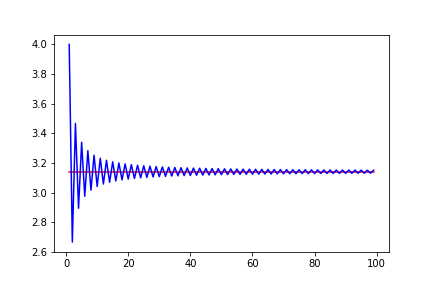
\includegraphics[scale=.75]{3c.png}
\end{center}
Here, $\pi$ is represented by the red line, and the blue line connects our approximations as the number of terms increases from 1 to 100. Due to the oscillatory nature of the polynomial, as well as the fact that the greater the number of terms, the smaller each contribution is, we see that this function converges quite slowly towards the true value.
\end{enumerate}
\item Consider the following expansions:
\begin{align*}
f(x+h) &= f(x)+hf'(x)+\frac{h^2}{2}f''(x)+\frac{h^3}{6}f'''(x)\\
f(x+2h) &= f(x)+2hf'(x)+\frac{4h^2}{2}f''(x)+\frac{8h^3}{6}f'''(x)
\end{align*}
Then,
\begin{align*}
4f(x+h)&=4f(x)+4hf'(x)+2h^2f''(x)+\frac{4h^3}{6}f'''(x)\\
-f(x+2h) &= -f(x)-2hf'(x)-\frac{4h^2}{2}f''(x)-\frac{8h^3}{6}f'''(x)
\end{align*}
So,
\[4f(x+h)-f(x)-f(x+2h) = 2hf'(x)-\frac{4h^3}{6}f'''(x)\]
Simplifying, and factoring the error term out,
\[2hf'(x)=4f(x+h)-f(x)-f(x+2h)+\frac{4h^3}{6}f'''(x)\]
\[f'(x)\approx \frac{4f(x+h)-f(x)-f(x+2h)}{2h}+\frac{h^2}{3}f'''(c)\]
Thus, we have the error term to be $\mathcal{O}(h^2)$ as desired.
\item Using $\mathcal{O}(h^2)$ approximations to approximate the derivative of the function contained in the file, we find the following approximations for each point of the interval,
\begin{align*}
L &= \frac{\frac{-3}{2}f(x_0)+2f(x_1)-\frac{1}{2}f(x_2)}{h}\\
C &= \frac{-\frac{1}{2}f(x_{k-1})+\frac{1}{2}f(x_{k+1})}{h}\\
R &= \frac{\frac{1}{2}f(x_{n-2})-2f(x_{n-1})+\frac{3}{2}f(x_n)}{h}
\end{align*}
Using Python, we actively compute the derivative over the data points, and plot it along side the original function. The results follow:
\begin{center}
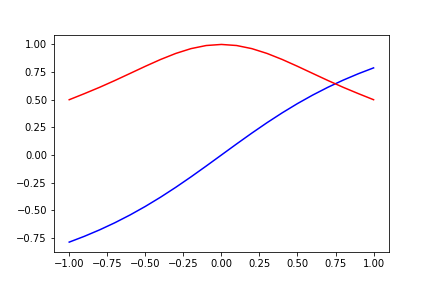
\includegraphics[scale=.75]{5.png}
\end{center}
With the original function in blue, and the derivative in red. As a check, we note that the derivative has a slope of $1$ at $x=0$. We plot the line $y=x$ to see if the function has this slope below,
\begin{center}
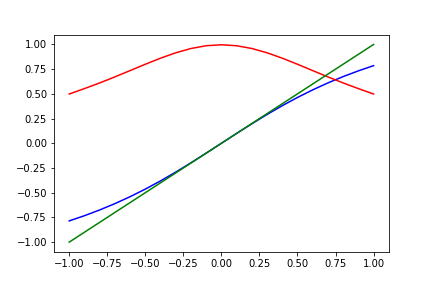
\includegraphics[scale=.75]{5b.png}
\end{center}
So, we see that our derivative function seems to be working as designed.
\item To approximate $\sqrt{R}$ for $R>1$, we consider the analagous function,
\[x^2-R=0\]
We then construct a newtons method regime to solve the analagous equation,
\[x^2-2=0\]
We know that $R>1$, and thus we pick our starting $x=1$. Setting our appropriate tolerance, we compute our approximate root to be,
\[\sqrt{2}\approx 1.4142135623746899\]
Using the built in numpy root function, we compute the true value to be,
\[\sqrt{2}\approx 1.4142135623730951\]
So, we see that our Newtons method actually turns out to be accurate to the order $10^{-12}$ in this case. This convergence makes sense due to the quadratic convergent nature of Newtons Method.
\item We now implement Newton's Method to solve the reciprocal problem using the formula,
\[x^{-1}-R=0\]
Our Newton iteration formula is then,
\[x_{n+1}=x_n-\frac{x_n^{-1}-R}{-x_n^{-2}}\]
Implementing in Jupyter Notebook, we compute the reciprocals to the first 5 integers to $10^{-8}$ accuracy to be,
\begin{align*}
1^-1 &= 0.9999999995283748\\
2^{-1} &= 0.4999999997641874\\
3^{-1} &= 0.33333333333332993\\
4^{-1} &= 0.24999999988209376\\
5^{-1} &= 0.19999999999956045\\
10^{-1} &= 0.09999999999978022
\end{align*}
We see that this implementation works quite well.
\item We consider the equation of absolute error in a Taylor polynomial,
\[|E|\leq \frac{M}{(n+1)!}|x-a|^{n+1}\]
First, we compute $M$ to be the maximum value of the $n+1$ derivative,
\[f^5(x)=\frac{105}{32}x^{9/2}\]
Over the interval $[\frac{1}{4},1]$, we see that the maximum value occurs at $x=1$. This becomes,
\[M=\frac{105}{32}\]
We then consider maximizing the $x-a$ term of the formula,
\[|x-a|=|x-\frac{9}{16}|\]
This is also maximized at $x=1$. Thus, our error is maximized at $1$ and the maximal value is then,
\[|E|\leq \frac{105}{32*5!}\bigg|\frac{7}{16}\bigg|^5\approx 4.382767\times10^{-4}\]
\item Consider $\vec{u},\ \vec{v}\in \R^n$. Consider now the following,
\begin{align*}
||\vec{u}+\vec{v}||^2 &= (\vec{u}+\vec{v})\cdot(\vec{u}+\vec{v}) && \text{The inner product}\\
&=||u||^2+2(\vec{u}\cdot \vec{v})+||v||^2 && \text{Note the Cauchy-Schwarz Inequality}\\
||u||^2+2(\vec{u}\cdot \vec{v})+||v||^2 &\leq ||u||^2+2(||\vec{u}||\ ||\vec{v}||)+||v||^2 && \text{Simplify}\\
&=(||u||+||v||)^2
\end{align*}
So,
\begin{align*}
||\vec{u}+\vec{v}||^2 &\leq (||u||+||v||)^2\\
&\Leftrightarrow\\
||\vec{u}+\vec{v}|| &\leq ||u||+||v||
\end{align*}
As desired.
\item We consider the Fresnel cosine function,
\[f(x)=\int_0^x\cos\big(\frac{\pi}{2}t^2\big)dt\]
To begin, we consider the Maclaurin expansion of cosine,
\[\cos(t)=\sum_{k=0}^{\infty}\frac{(-1)^kt^{2k}}{(2k)!}\]
Substituting our fresnel cosine parenthesis,
\[\cos\big(\frac{\pi}{2}t^2\big)=\sum_{k=0}^{\infty}\frac{(-1)^k\big(\frac{\pi}{2}t^2\big)^{2k}}{(2k)!}=\sum_{k=0}^{\infty}\frac{(-1)^k\pi^{2k}t^{4k}}{2^{2k}(2k)!}\]
Finally, we apply the integral operator,
\begin{align*}
\int_0^x\cos\big(\frac{\pi}{2}t^2\big)dt&=\int_0^x\sum_{k=0}^{\infty}\frac{(-1)^k\pi^{2k}t^{4k}}{2^{2k}(2k)!}dt\\
&=\sum_{k=0}^{\infty}\frac{(-1)^k\pi^{2k}x^{4k+1}}{(4k+1)2^{2k}(2k)!}
\end{align*}
We note that due to the polynomial nature of the series, we may completely drop the lower bound of the integrand, as the polynomial will always be identically zero. Thus, our sum need only be evaluated at $x$. Thus,
\[f(x)= x-\frac{\pi^2x^5}{(5)(4)(2)}+\ldots\]
And,
\[f(1)\approx 1-\frac{\pi^2(1)}{40}=0.753259889972766\]
To compute the maximum error of $f(x)$ from above, we consider the maximal value of the next term in the sequence over the interval $[0,1]$. This is because the only non-zero terms in the polynomial expansions are those that contain $\cos(\pi t^2/2)$, whose maximum is at $1$. The error then becomes,
\[|E|\leq\frac{f^{n+1}(c)}{(n+1)!}(x-x_0)^{n+1}\]
This term is,
\[|E|\leq\frac{\pi^4}{(9)(2^4)(4!)}\approx 0.0281855009\]
Finally, we consider how many terms would be necessary to reach machine precision with $f(1)$. We consider what machine epsilon means. This is the smallest number that the computer can accurately represent. As such, we need to find the first term that is less than machine epsilon. Running a while look in Python, we find that the tenth term of the expansion is less than machine epsilon. Thus, we can compute the degree of the term as,
\[x^{4(10)+1}=x^{41}\]
So the degree for machine precision on $f(1)$ is $41$.\\
Looking at the built in plotting functionality of the fresnel function, we compare it to both the $2$ and $3$ term expansion of our integral, and overlay the plots as follows:
\begin{center}
For $n=2$ terms,\\
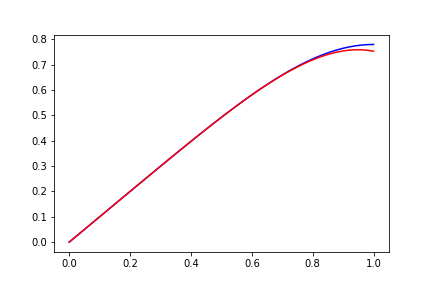
\includegraphics[scale=.65]{10a.png}\\
For $n=3$ terms,\\
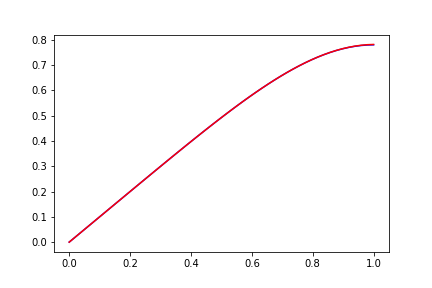
\includegraphics[scale=.65]{10b.png}
\end{center}
We see that the approximation (red) has its greatest error at the right point of the interval, which makes sense, as our Maclaurin series is centered at $0$, so the error in our approximation increases the further away from $0$. As we increase the number of terms from $n=2$ to $n=3$, we see that the approximation increases in accuracy as we would expect.
\end{enumerate}
\end{document}
